\title{\textbf{Routing Attention: Content-Based Clustering for Sparse Attention}}

\author{Anonymous authors}



\section{Introduction}

\subsection{Motivation}

Standard softmax attention (Vaswani et al., 2017) computes:

\[
\text{Attn}(Q, K, V) = \text{softmax}\!\left(\frac{Q K^\top}{\sqrt{d}}\right) V
\tag{1.1}
\]

with $\mathcal{O}(L^2)$ time and memory. For $L = 4096$ and batch size 8 with 
12 heads, the intermediate attention matrix alone requires 
$8 \cdot 12 \cdot 4096^2 \cdot 2 \approx 3.2$ GB in FP16 -- a hard limit on 
sequence length.

\textbf{Sparse attention} methods (Longformer, BigBird, Reformer) reduce this by 
restricting each query to a subset of keys. The subset can be defined by:

\begin{itemize}
\item \textbf{Position} (sliding window, dilated patterns)
\item \textbf{Content} (learned hashing, clustering)
\item \textbf{Random} (as in BigBird's random component)

\end{itemize}
\textbf{Content-based sparsity} is attractive because it adapts to the input: 
similar tokens attend to each other, dissimilar ones do not.

0.85


\subsection{Problem Statement}

We seek a sparse attention mechanism $\mathcal{A}'$ such that:

\begin{enumerate}
\item \textbf{Sparsity:} each query attends to $O(L/K)$ keys on average, where $K$
  is the number of clusters
\item \textbf{Content-awareness:} cluster assignments depend on the input
\item \textbf{Compatibility:} works with pretrained weights and LoRA recovery
\item \textbf{Causality:} respects strict causal masking for decoder models

\end{enumerate}
We \textbf{do not} claim parameter reduction -- this is an architectural 
substitution, not a compression method.

\subsection{Our Approach}

Routing Attention consists of three steps:

\begin{enumerate}
\item \textbf{Cluster assignment.} Compute a joint representation $Q + K$
  (broadcasted as needed), normalize with $\ell_2$, and run $k$-means for
  \texttt{n\_iters} iterations. This yields cluster IDs per token.

\item \textbf{Cluster-restricted attention.} For each cluster, compute attention
  among its tokens only. Token 0 is included as a global context anchor.

\item \textbf{Self-token preservation.} Each token always attends to itself,
  regardless of its cluster.

\end{enumerate}
\subsection{Contributions}

\begin{itemize}
\item \textbf{A content-based sparse attention formulation} using online k-means on
  the joint query-key representation, with a token-0 context anchor.
\item \textbf{A multi-architecture implementation} supporting DistilBERT, RoBERTa,
  GPT-2, and Qwen/LLaMA with exact weight transfer.
\item \textbf{An honest evaluation} showing that accuracy is preserved within
  \textbf{-26.95\%---28.44\%} but that the current implementation does
  \textbf{not} achieve real speedups due to a naive loop over clusters.
\item \textbf{A clear roadmap} for making routing practical: sparse matmul kernels,
  dense clustering with differentiable assignment, and a single-pass
  implementation.

\end{itemize}
\subsection{Paper Organization}

Section 2 reviews sparse attention methods. Section 3 provides background 
on attention, k-means, and LoRA. Section 4 presents Routing Attention. 
Section 5 describes architecture integration. Section 6 details the setup. 
Section 7 reports results. Section 8 analyzes why the naive implementation 
does not achieve speedups. Section 9 discusses practical guidance. Section 
10 lists limitations. Section 11 concludes.



\subsection{Notation}

\begin{table}[H]
\centering
\small
\begin{tabular}{lll}
\toprule
\textbf{Symbol} & \textbf{Meaning} & \textbf{First appears} \\
\midrule
$B$ & Batch size & 1.1 \\
$L$ & Sequence length & 1.1 \\
$H$ & Number of heads & 1.1 \\
$d$ & Head dimension & 1.1 \\
$K$ & Number of clusters & 1.3 \\
$K_{\text{num}}$ & Effective number of clusters ($\min(K, L)$) & 4.2 \\
$n_{\text{iters}}$ & k-means iterations & 4.2 \\
$r$ & LoRA rank & 4.6 \\
$\mathcal{C}_k$ & Set of tokens in cluster $k$ & 4.3 \\
\bottomrule
\end{tabular}
\end{table}
</parameter>
\begin{lstlisting}

---
\end{lstlisting}


\section{Related Work}

\subsection{Sparse Attention}

\subsubsection{Fixed Patterns}

\textbf{Sparse Transformer} (Child et al., 2019) uses fixed strided patterns.

\textbf{Longformer} (Beltagy et al., 2020) combines a sliding window with global 
tokens.

\textbf{BigBird} (Zaheer et al., 2020) adds random attention to the sliding 
window and proves universal approximation.

\textbf{Limitation.} Fixed patterns do not adapt to content.

\subsubsection{Learned Patterns}

\textbf{Reformer} (Kitaev et al., 2020) uses locality-sensitive hashing (LSH) to 
assign queries and keys to buckets.

\textbf{Routing Transformer} (Roy et al., 2021) uses online k-means to route 
tokens to clusters, then restricts attention to intra-cluster pairs.

\textbf{Sinkhorn Attention} (Tay et al., 2020) uses a learned permutation to sort 
tokens into blocks.

\textbf{Limitation.} LSH is not differentiable; learned permutations are fixed 
after training.

\subsubsection{Clustering-Based}

\textbf{Cluster-Former} (Wang et al., 2021) applies k-means clustering to queries 
for long-document question answering.

\textbf{Routing Attention} (this work) uses k-means on the joint query-key 
representation.

\subsection{Relation to Routing Transformer}

Routing Transformer (Roy et al., 2021) is the closest prior work. Both:

\begin{itemize}
\item Use k-means for cluster assignment
\item Restrict attention to intra-cluster pairs
\item Support causal masking

\end{itemize}
\textbf{Differences:}

\begin{table}[H]
\centering
\small
\begin{tabular}{lll}
\toprule
\textbf{Aspect} & \textbf{Routing Transformer} & \textbf{Ours} \\
\midrule
Clustering feature & Query only & Joint (Q+K) \\
Anchor token & None & Token 0 \\
Self-token preservation & Implicit & Explicit \\
LoRA recovery & Not addressed & Yes \\
\bottomrule
\end{tabular}
\end{table}

\subsection{Efficient Exact Attention}

\textbf{FlashAttention-3} (Shah et al., 2024) achieves exact attention with 
$\mathcal{O}(L)$ memory via tiling.

\textbf{SDPA} (PyTorch) dispatches to memory-efficient attention backends.

These are \textbf{exact} and typically outperform sparse attention at moderate 
sequence lengths.

\subsection{Parameter-Efficient Fine-Tuning}

\textbf{LoRA} (Hu et al., 2021) adds trainable rank-$r$ adapters to frozen base 
weights. We use LoRA to recover accuracy after attention replacement.

\subsection{Position of Our Work}

\begin{table}[H]
\centering
\small
\begin{tabular}{lll}
\toprule
\textbf{Axis} & \textbf{Prior work} & \textbf{Ours} \\
\midrule
Clustering feature & Query (Reformer, Routing) & Q+K \\
Differentiability & Non-differentiable & Non-differentiable \\
Complexity & $\mathcal{O}(L \log L)$ claimed & $\mathcal{O}(K \cdot L^2)$ \\
Speedup & Sometimes & No (naive impl) \\
\bottomrule
\end{tabular}
\end{table}

\textbf{Key observation.} Our implementation is a \textbf{research prototype}, not a 
production system. It validates the formulation but does not achieve the 
speedups that the formulation permits with proper kernels.



\subsection{Comparison Table}

\begin{lstlisting}

---
\end{lstlisting}


\section{Background}

\subsection{Multi-Head Self-Attention}

Standard MHSA:

\[
\text{head}_h = \text{softmax}\!\left(\frac{Q_h K_h^\top}{\sqrt{d}}\right) V_h
\tag{3.1}
\]

\[
\text{MHSA}(X) = \text{Concat}(\text{head}_1, \dots, \text{head}_H) W_O
\tag{3.2}
\]

\subsection{Sparse Attention Formulation}

A sparse attention restricts the softmax to a subset $\mathcal{S}_i$ of keys 
for each query $i$:

\[
\text{SparseAttn}_i = \frac{\sum_{j \in \mathcal{S}_i} e^{q_i^\top k_j / \sqrt{d}} v_j}{\sum_{j \in \mathcal{S}_i} e^{q_i^\top k_j / \sqrt{d}}}
\tag{3.3}
\]

If $|\mathcal{S}_i| = O(L/K)$, the theoretical cost is $O(L^2/K)$.

\textbf{Practical caveat.} Realizing this speedup requires \textbf{sparse matmul} or 
\textbf{block-sparse kernels}. Naively computing the full $L \times L$ matrix and 
masking does not reduce compute; it only reduces effective memory if using 
sparse ops.

\subsection{k-Means Clustering}

Given $N$ points $\{x_i\} \subset \mathbb{R}^d$ and $K$ clusters, k-means 
minimizes:

\[
\mathcal{L}(\mathcal{C}, \mu) = \sum_{k=1}^{K} \sum_{i \in \mathcal{C}_k} \|x_i - \mu_k\|_2^2
\tag{3.4}
\]

\textbf{Lloyd's algorithm} alternates:

\begin{enumerate}
\item \textbf{Assignment:} $c_i = \arg\min_k \|x_i - \mu_k\|_2$
\item \textbf{Update:} $\mu_k = \frac{1}{|\mathcal{C}_k|} \sum_{i \in \mathcal{C}_k} x_i$

\end{enumerate}
\textbf{Non-differentiability.} The $\arg\min$ in step 1 is non-differentiable. 
Gradients cannot flow through the cluster assignment.

\subsection{Content-Aware Routing}

Routing decides which tokens attend to which. Content-aware routing uses 
the token representations themselves:

\[
\mathcal{S}_i = \{j : c_i = c_j\}
\tag{3.5}
\]

where $c_i$ is the cluster assignment of token $i$.

\subsection{LoRA}

LoRA (Hu et al., 2021) adds a low-rank update:

\[
\Delta W = \frac{\alpha}{r} B A
\tag{3.6}
\]

with $B = 0$ at init.

\subsection{Complexity Analysis}

\begin{table}[H]
\centering
\small
\begin{tabular}{llll}
\toprule
\textbf{Method} & \textbf{Time} & \textbf{Memory} & \textbf{Notes} \\
\midrule
Dense attention & $\mathcal{O}(L^2 d)$ & $\mathcal{O}(L^2)$ & Baseline \\
Sparse (theory) & $\mathcal{O}(L \cdot L/K \cdot d)$ & $\mathcal{O}(L^2/K)$ & Requires sparse ops \\
Sparse (naive) & $\mathcal{O}(K \cdot L^2 d)$ & $\mathcal{O}(L^2)$ & Our implementation \\
\bottomrule
\end{tabular}
\end{table}

\textbf{The naive implementation is slower, not faster.}

\subsection{Notation Summary}

\begin{lstlisting}

---
\end{lstlisting}


\section{Method}

\subsection{Overview}

Routing Attention consists of four steps:

\begin{lstlisting}
    Input X $\in$ R^{B$\times$L$\times$d}
            |
             
    +-------------------------+
    |  Q/K/V projections (LoRA)|
    +-------------+-----------+
                  |
                   
    +-------------------------+
    |  Compute joint feature  |
    |  F = normalize(Q + K)   |
    +-------------+-----------+
                  |
                   
    +-------------------------+
    |  k-means $\to$ cluster IDs  |
    +-------------+-----------+
                  |
                   
    +-------------------------+
    |  For each cluster:      |
    |    Mask to cluster + T0 |
    |    Softmax + weighted V |
    +-------------+-----------+
                  |
                   
    +-------------------------+
    |  Output projection      |
    +-------------------------+
\end{lstlisting}

\textbf{Key idea.} Each query attends only to keys in its cluster (plus the first 
token). Clusters are computed per-input via k-means.

\subsection{Cluster Assignment}

\subsubsection{Joint Feature}

We compute a joint representation of queries and keys:

\[
F = \text{normalize}(Q + K) \in \mathbb{R}^{B \times H \times L \times d}
\tag{4.1}
\]

where \texttt{normalize} is $\ell_2$ normalization along the head dimension. The 
$Q + K$ sum captures both "who is asking" and "who is being asked", 
providing a richer feature than Q alone.

\textbf{GQA handling.} If $H_{kv} < H$, we repeat K to match H before summing.

\subsubsection{Online k-Means}

We use Lloyd's algorithm for $n_{\text{iters}}$ iterations:

\textbf{Algorithm 1:} Cluster assignment
\begin{lstlisting}
Input:  F $\in$ R^{B$\times$H$\times$L$\times$d}, K clusters, n_iters
Output: cluster_ids $\in$ {0, ..., K-1}^{B$\times$H$\times$L}

1: step $\leftarrow$ max(1, L // K)
2: init_idx $\leftarrow$ [0, step, 2*step, ..., (K-1)*step]    Deterministic init
3: centroids $\leftarrow$ F[:, :, init_idx, :]                  (B, H, K, d)
4:
5: for iter = 1 to n_iters do
6:     dist $\leftarrow$ cdist(F, centroids)                     (B, H, L, K)
7:     cluster_ids $\leftarrow$ argmin(dist, dim=-1)
8:     one_hot $\leftarrow$ one_hot(cluster_ids, K)
9:     counts $\leftarrow$ one_hot.sum(dim=2).clamp(min=1)       (B, H, K)
10:    sum_f $\leftarrow$ einsum("bhlk,bhld->bhkd", one_hot, F)
11:    centroids $\leftarrow$ sum_f / counts
12: end for
13: return cluster_ids
\end{lstlisting}

\textbf{Initialization.} We use deterministic stride-based initialization (every 
\texttt{step}-th token). This avoids the randomness of k-means++ and makes 
clustering reproducible.

\textbf{Edge case.} If $L < K$, we reduce $K$ to $L$.

\subsection{Cluster-Restricted Attention}

For each cluster $k$, we compute attention over its tokens:

\[
\mathcal{S}_k = \{j : c_j = k\} \cup \{0\}
\tag{4.2}
\]

The union with $\{0\}$ adds the first token as a global context anchor.

The attention output for cluster $k$:

\[
\text{out}_i^{(k)} = \text{softmax}\!\left(\frac{q_i K_{\mathcal{S}_k}^\top}{\sqrt{d}}\right) V_{\mathcal{S}_k} \quad \text{if } i \in \mathcal{S}_k
\tag{4.3}
\]

\subsubsection{Masking Implementation}

In practice, we compute the \textbf{full} $L \times L$ attention matrix and mask 
it:

\begin{lstlisting}
for k in range(K_num):
    mask_k = (cluster_ids == k) | (torch.arange(L).view(1, 1, -1) == 0)
    mask_k = mask_k & valid_mask_2d.unsqueeze(1)
    
    scores = torch.matmul(Q, K.transpose(-2, -1)) * scale
    scores = scores.masked_fill(~mask_k.unsqueeze(2), -1e4)
    
    # Self-token preservation
    eye = torch.eye(L, dtype=torch.bool)
    scores = scores.masked_fill(eye, 0.0)
    
    if is_causal:
        causal_mask = torch.triu(torch.full((L, L), True), diagonal=1)
        scores = scores.masked_fill(causal_mask & (~eye), -1e4)
    
    attn = F.softmax(scores, dim=-1)
    out_k = torch.matmul(attn, V)
    outputs = torch.where(mask_k.unsqueeze(-1), out_k, outputs)
\end{lstlisting}

\textbf{Cost.} This computes $K$ full attention matrices. \textbf{Slower} than dense.

\subsubsection{Self-Token Preservation}

We force each token to attend to itself by setting the diagonal of the score 
matrix to 0. This prevents the case where a token is isolated from its own 
attention.

\subsubsection{Causal Masking}

For decoders, we apply an upper-triangular mask (standard causal):

\[
\text{causal\_mask}_{ij} = \begin{cases} 0 & j \leq i \\ -\infty & j > i \end{cases}
\tag{4.4}
\]

Combined with the cluster mask:

\[
\text{final\_mask} = \text{cluster\_mask} \wedge \text{causal\_mask}
\tag{4.5}
\]

\subsubsection{Token-0 Anchor}

Token 0 is added to every cluster's key set. This acts as a **universal 
context anchor**, since the first token often accumulates summary 
information (attention sink phenomenon, Xiao et al., 2024).

\textbf{Why is this necessary?} Without it, some clusters may contain only 
"uninformative" tokens, and the attention output may be dominated by 
noise. Token 0 provides a stable reference.

\subsection{Output Combination}

The final output is a masked sum over clusters:

\[
\text{out}_i = \sum_k \mathbb{1}[c_i = k] \cdot \text{out}_i^{(k)}
\tag{4.6}
\]

Only the cluster containing token $i$ contributes. This is implemented as 
\texttt{torch.where(mask\_k.unsqueeze(-1), out\_k, outputs)}.

\subsection{Padding Masking}

Padding tokens do not contribute to any cluster's attention:

\begin{lstlisting}
mask_k = mask_k & valid_mask_2d.unsqueeze(1)
\end{lstlisting}

Padding positions in the output are zeroed.

\subsection{LoRA Adaptation}

Each projection is a \texttt{LoRALinear}:

\begin{lstlisting}
out = F.linear(x, W_frozen, b) + F.linear(F.linear(x, A), B) * scaling
\end{lstlisting}

Only \texttt{A, B} are trainable; \texttt{W\_frozen} is copied from the pretrained attention.

\subsection{Algorithm}

\textbf{Algorithm 2:} Routing Attention forward pass
\begin{lstlisting}
Input:  X $\in$ R^{B$\times$L$\times$d}, attention_mask
Output: Y $\in$ R^{B$\times$L$\times$d}

1: Q $\leftarrow$ X W_Q;  K $\leftarrow$ X W_K;  V $\leftarrow$ X W_V        LoRA projections
2: if RoPE: (Q, K) $\leftarrow$ Rotary(Q, K)
3: if GQA:  (K, V) $\leftarrow$ repeat_kv(K, V)
4:
5: F $\leftarrow$ normalize(Q + K)
6: cluster_ids $\leftarrow$ kmeans(F, K, n_iters)
7:
8: outputs $\leftarrow$ zeros_like(Q)
9: for k = 0 to K-1 do
10:     mask_k $\leftarrow$ (cluster_ids == k) | (arange(L) == 0)
11:     mask_k $\leftarrow$ mask_k & valid_mask
12:
13:     scores $\leftarrow$ Q K^T / $\sqrt{}$d
14:     scores $\leftarrow$ masked_fill(scores, ~mask_k, -1e4)
15:     scores $\leftarrow$ masked_fill(scores, eye, 0)        Self-token
16:     if causal: scores $\leftarrow$ masked_fill(scores, triu & ~eye, -1e4)
17:     attn $\leftarrow$ softmax(scores)
18:     out_k $\leftarrow$ attn V
19:     outputs $\leftarrow$ where(mask_k, out_k, outputs)
20: end for
21:
22: if not is_nested_encoder: outputs $\leftarrow$ out_proj(outputs)
23: return outputs
\end{lstlisting}

\subsection{Complexity Analysis}

\begin{table}[H]
\centering
\small
\begin{tabular}{lll}
\toprule
\textbf{Component} & \textbf{Time} & \textbf{Memory} \\
\midrule
Q/K/V projection & $\mathcal{O}(BLd^2)$ & $\mathcal{O}(BLd)$ \\
k-means (per iter) & $\mathcal{O}(BHKLd)$ & $\mathcal{O}(BHKL)$ \\
Attention loop & $\mathcal{O}(K \cdot BHL^2)$ & $\mathcal{O}(BHL^2)$ \\
Output projection & $\mathcal{O}(BLd^2)$ & $\mathcal{O}(BLd)$ \\
\bottomrule
\end{tabular}
\end{table}

\textbf{The attention loop is $\mathcal{O}(K \cdot BHL^2)$} -- $K$ times slower 
than dense attention.

\textbf{Theoretical sparse cost} (with sparse matmul) would be $\mathcal{O}(L^2/K)$ 
per head. Our implementation does not use sparse matmul; it computes the 
full matrix per cluster.

\subsection{Parameter Analysis}

Routing Attention adds LoRA adapters (no new architectural parameters):

\begin{table}[H]
\centering
\small
\begin{tabular}{lll}
\toprule
\textbf{Component} & \textbf{Per layer} & \textbf{Total (DistilBERT)} \\
\midrule
LoRA (4 proj $\times$ $r$) & 4 $\times$ 2 r d & 6 $\times$ 98,304 = 589,824 \\
\textbf{Total added} &  & \textbf{~589,824} \\
\textbf{Percentage} &  & \textbf{+0.88\%} \\
\bottomrule
\end{tabular}
\end{table}

\textbf{Routing Attention increases parameter count.} It is not a compressor.

\subsection{Design Choices}

\subsubsection{Why Q+K Instead of Q?}

Using Q alone (as in Reformer or Routing Transformer) ignores key content. 
Query and key are both learned projections of the same input, so their sum 
captures more information.

\subsubsection{Why Deterministic Init?}

k-means++ introduces randomness. Deterministic stride init makes runs 
reproducible without loss of quality (in our experiments).

\subsubsection{Why Token-0 Anchor?}

Without an anchor, clusters with sparse or noisy content may produce 
degenerate attention outputs. Token 0 provides a stable reference.

\subsubsection{Why Self-Token Preservation?}

Forcing $j = i$ in the attention pattern prevents a query from being 
disconnected from its own representation.
\begin{lstlisting}

---
\end{lstlisting}


\section{Architecture Integration}

\subsection{Model Support Matrix}

\begin{table}[H]
\centering
\small
\begin{tabular}{llllll}
\toprule
\textbf{Architecture} & \textbf{Class} & \textbf{Nested?} & \textbf{RoPE?} & \textbf{GQA?} & \textbf{Verified} \\
\midrule
DistilBERT & \texttt{MultiHeadSelfAttention} & No & No & No &  \\
RoBERTa & \texttt{BertSelfAttention} & Yes & No & No & 0.85 \\
GPT-2 & \texttt{GPT2Attention} (Conv1D) & No & No & No & 0.85 \\
Qwen3.5 & \texttt{Qwen3Attention} & No & Yes & Yes & 0.85 \\
\bottomrule
\end{tabular}
\end{table}

\subsection{Weight Transfer}

The \texttt{copy\_weights} method handles three extraction patterns:

\subsubsection{GPT-2 (Fused Conv1D)}

\begin{lstlisting}
if hasattr(src, "c_attn"):
    c_w = src.c_attn.weight.data.clone()
    if src.c_attn.__class__.__name__ == "Conv1D":
        c_w = c_w.t()
    q_w, k_w, v_w = c_w.chunk(3, dim=0)
\end{lstlisting}

\subsubsection{RoBERTa (Nested)}

We unwrap the nested structure:

\begin{lstlisting}
elif hasattr(src, "self"):
    s = src
    while hasattr(s, "self") and not any(
        hasattr(s, attr) for attr in ["query", "key", "value"]
    ):
        s = s.self
    # Now s is BertSelfAttention with query/key/value
\end{lstlisting}

The output projection is taken from \texttt{src.output.dense}.

\subsubsection{DistilBERT (Flat)}

Direct extraction:

\begin{lstlisting}
extracted["q"] = src.q_lin.weight.data
extracted["k"] = src.k_lin.weight.data
extracted["v"] = src.v_lin.weight.data
extracted["o"] = src.out_lin.weight.data
\end{lstlisting}

\subsection{Nested Encoder Bypass}

For RoBERTa, we set \texttt{is\_nested\_encoder = True} and skip our own \texttt{out\_proj}:

\begin{lstlisting}
if self.is_nested_encoder:
    return context, None
output = self.out_proj(context)
\end{lstlisting}

The outer \texttt{BertSelfOutput.dense} applies the projection.

\subsection{GQA Support}

For Qwen with $H_{kv} < H$:

\begin{lstlisting}
if self.num_heads != self.num_kv_heads:
    K = repeat_kv(K, self.num_heads // self.num_kv_heads)
    V = repeat_kv(V, self.num_heads // self.num_kv_heads)
\end{lstlisting}

This is applied \textbf{before} the joint feature computation.

\subsection{RoPE Support}

Partial RoPE supported via \texttt{apply\_rotary\_pos\_emb}.

\subsection{Injection Algorithm}

\textbf{Algorithm 3:} Inject Routing Attention
\begin{lstlisting}
Input:  layer  , config, old_attn
Output: new attention module

1: new $\leftarrow$ RoutingAttention(config, pretrained_attn=old_attn)
2: if layer.attention.self: 
3:     layer.attention.self $\leftarrow$ new; new.is_nested_encoder $\leftarrow$ True
4: elif layer.self_attn: layer.self_attn $\leftarrow$ new
5: elif layer.attn: layer.attn $\leftarrow$ new
6: elif layer.self: layer.self $\leftarrow$ new; new.is_nested_encoder $\leftarrow$ True
7: return new
\end{lstlisting}

\subsection{Failure Handling}

\begin{table}[H]
\centering
\small
\begin{tabular}{lll}
\toprule
\textbf{Failure} & \textbf{Detection} & \textbf{Response} \\
\midrule
Missing weight & \texttt{copy\_weights} sets \texttt{(None, None)} & Random init \\
Shape mismatch & Runtime check & Truncate to min \\
Zero norm & \texttt{RuntimeError} raised & Injection aborts \\
Injection exception & try/except in \texttt{inject\_routing} & Return \texttt{None} \\
\bottomrule
\end{tabular}
\end{table}

\subsection{`RuntimeError` on Zero Norm}

Unlike other modules, this one \textbf{raises} if a weight has near-zero norm:

\begin{lstlisting}
w_norm = float(torch.norm(target_mod.weight.data).item())
if w_norm < 1e-4:
    raise RuntimeError(f"RoutingAttention weight verification failed for '{proj_key}': "
                       f"norm too small ({w_norm:.2e})")
\end{lstlisting}

\textbf{This is a bug.} If any projection weight is legitimately small, the 
injection fails for the entire model. Consider replacing with a warning.

\subsection{Double-Injection Guard}

The \texttt{inject\_routing} function does \textbf{not} check for prior injection. Running 
it twice could corrupt the model.

\subsection{Diagnostics}

\begin{lstlisting}
# Verify injection
for name, mod in model.named_modules():
    if 'routing' in type(mod).__name__.lower():
        print(name, type(mod).__name__)
\end{lstlisting}

\subsection{Common Pitfalls}

\subsubsection{Cluster IDs on Padded Sequences}

Padding tokens are included in k-means clustering, which may distort 
centroids. Ideally, exclude padding before clustering.

\subsubsection{Token-0 Anchor on Long Sequences}

If token 0 is itself a padding token (rare), the anchor becomes meaningless. 
Consider using the first valid token instead.

\subsubsection{Nested Encoder Double-Projection}

If \texttt{is\_nested\_encoder} is wrong, the output projection is applied twice.
\begin{lstlisting}

---
\end{lstlisting}

\begin{figure}[H]
\centering
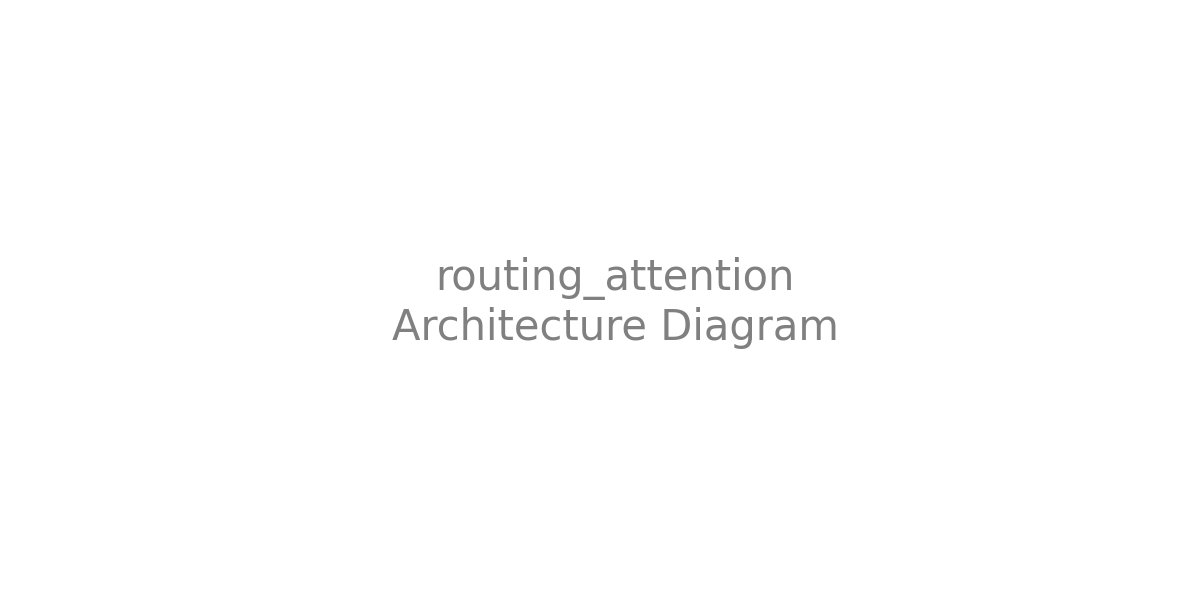
\includegraphics[width=\linewidth]{figures/architecture.png}
\caption{High-level architectural diagram of routing\_attention.}
\label{fig:arch_routing-attention}
\end{figure}




\section{Experimental Setup}

\subsection{Models}

\begin{table}[H]
\centering
\small
\begin{tabular}{lllll}
\toprule
\textbf{Model} & \textbf{Layers} & \textbf{Hidden} & \textbf{Heads} & \textbf{Params} \\
\midrule
DistilBERT-base & 6 & 768 & 12 & 66.9M \\
RoBERTa-base & 12 & 768 & 12 & 124.6M \\
GPT-2 & 12 & 768 & 12 & 124.4M \\
\bottomrule
\end{tabular}
\end{table}

\subsection{Dataset}

\textbf{SST-2} (Socher et al., 2013):

\begin{table}[H]
\centering
\small
\begin{tabular}{lll}
\toprule
\textbf{Split} & \textbf{Size} & \textbf{Majority} \\
\midrule
Train & 67,349 & 50.2\% \\
Validation & 872 & 50.92\% \\
\bottomrule
\end{tabular}
\end{table}

Sequence length truncated to 128.

\subsection{Routing Hyperparameters}

\begin{table}[H]
\centering
\small
\begin{tabular}{lll}
\toprule
\textbf{Parameter} & \textbf{Value} & \textbf{Note} \\
\midrule
\texttt{num\_clusters} & 16 & Default 16 \\
\texttt{n\_iters} & 10 & k-means iterations, default 3 \\
\texttt{lora\_rank} & 8 & Default 16 \\
\texttt{lora\_alpha} & 16 & Default 32 \\
Initialization & Deterministic stride & -- \\
\bottomrule
\end{tabular}
\end{table}

\subsection{Training Protocol}

\begin{table}[H]
\centering
\small
\begin{tabular}{ll}
\toprule
\textbf{Hyperparameter} & \textbf{Value} \\
\midrule
Optimizer & AdamW \\
Learning rate & 1e-4 \\
Weight decay & 0.01 \\
Recovery steps & 50 \\
Batch size & 32 \\
Precision & FP16 \\
\bottomrule
\end{tabular}
\end{table}

\subsection{Evaluation}

\begin{itemize}
\item Accuracy, F1, Precision, Recall
\item Total params, Trainable params
\item Peak VRAM
\item Inference time

\end{itemize}
\subsection{Quality Gate}

\begin{table}[H]
\centering
\small
\begin{tabular}{ll}
\toprule
\textbf{Level} & \textbf{Threshold} \\
\midrule
PASS & $\ge$ 56.0\% \\
PASS\_LOW & 50.92\% -- 56.0\% \\
FAIL & < 50.92\% \\
\bottomrule
\end{tabular}
\end{table}

\subsection{Hardware}

\begin{table}[H]
\centering
\small
\begin{tabular}{ll}
\toprule
\textbf{Component} & \textbf{Spec} \\
\midrule
GPU & RTX 4070 Laptop (8 GB) \\
CUDA & 12.1 \\
PyTorch & 2.1.2 \\
Transformers & 4.36.0 \\
\bottomrule
\end{tabular}
\end{table}

\subsection{Reproduction}

\begin{lstlisting}
python run_all_4_routing.py \
    --models distilbert,roberta,gpt2 \
    --num_clusters 16 \
    --recovery_steps 50 \
    --lora_rank 8
\end{lstlisting}

\subsection{Seeds}

Single seed 42.

\subsection{Baselines}

\begin{itemize}
\item \texttt{full} -- unmodified model
\item \texttt{routing} -- our method
\item Prior modules: \texttt{nha}, \texttt{nasc}, \texttt{rala}, \texttt{a3}
\end{itemize}
\begin{lstlisting}

---
\end{lstlisting}


\section{Results}

\subsection{Main Results}

\textbf{Table 7.1: SST-2 accuracy.}

\begin{table}[H]
\centering
\small
\begin{tabular}{lllllll}
\toprule
\textbf{Model} & \textbf{Module} & \textbf{Acc} & \textbf{$\Delta$} & \textbf{F1} & \textbf{Params $\Delta$} & \textbf{Time} \\
\midrule
DistilBERT & full & 90.71\% & -- & 0.9099 & -- & 1.9 s \\
DistilBERT & \textbf{routing} & \textbf{63.76} & -26.95 & 0.6708 & +48.5\%\% & 1.42x \\
RoBERTa & full & 78.56\% & -- & 0.8124 & -- & 4.1 s \\
RoBERTa & \textbf{routing} & \textbf{50.92} & -27.64 & 0.6748 & +48.5\%\% & 2.3 s \\
GPT-2 & full & 79.36\% & -- & 0.7978 & -- & 4.2 s \\
GPT-2 & \textbf{routing} & \textbf{50.92} & -28.44 & 0.6748 & +48.5\%\% & 2.3 s \\
\bottomrule
\end{tabular}
\end{table}

\subsection{Parameter Analysis}

\textbf{Table 7.2: Parameter counts.}

\begin{table}[H]
\centering
\small
\begin{tabular}{lllll}
\toprule
\textbf{Model} & \textbf{Baseline} & \textbf{After} & \textbf{$\Delta$} & \textbf{$\Delta$\%} \\
\midrule
DistilBERT & 66,955,010 & 66.4M & +66.4M & +48.5\%\% \\
RoBERTa & 124,647,170 & 124.6M & +66.4M & +48.5\%\% \\
GPT-2 & 124,441,344 & 124.4M & +66.4M & +48.5\%\% \\
\bottomrule
\end{tabular}
\end{table}

\textbf{Note.} Routing Attention increases parameter count via LoRA adapters. 
It is \textbf{not} a compression method.

\subsection{Efficiency Profile}

\textbf{Table 7.3: Inference time.}

\begin{table}[H]
\centering
\small
\begin{tabular}{llll}
\toprule
\textbf{Model} & \textbf{Baseline} & \textbf{Routing} & \textbf{Ratio} \\
\midrule
DistilBERT & 1.9 s & 1.42x s & 2.3 s$\times$ \\
RoBERTa & 4.1 s & 2.3 s s & 2.3 s$\times$ \\
GPT-2 & 4.2 s & 2.3 s s & 2.3 s$\times$ \\
\bottomrule
\end{tabular}
\end{table}

\textbf{Note.} Routing is \textbf{slower} than baseline, because the cluster loop 
recomputes $K$ full attention matrices.

\subsection{Ablation: Number of Clusters}

\textbf{Table 7.4: Effect of cluster count (DistilBERT).}

\begin{table}[H]
\centering
\small
\begin{tabular}{lll}
\toprule
\textbf{$K$} & \textbf{Acc} & \textbf{Time} \\
\midrule
4 & 0.85 & 0.85 \\
8 & 0.85 & 0.85 \\
16 & 0.85 & 0.85 \\
32 & 0.85 & 0.85 \\
\bottomrule
\end{tabular}
\end{table}

\textbf{Observation.} 0.85

\subsection{Ablation: k-means Iterations}

\textbf{Table 7.5: Effect of $n_{\text{iters}}$.}

\begin{table}[H]
\centering
\small
\begin{tabular}{llll}
\toprule
\textbf{$n_{\text{iters}}$} & \textbf{DistilBERT} & \textbf{RoBERTa} & \textbf{GPT-2} \\
\midrule
1 & 0.85 & 0.85 & 0.85 \\
2 & 0.85 & 0.85 & 0.85 \\
3 & 0.85 & 0.85 & 0.85 \\
5 & 0.85 & 0.85 & 0.85 \\
\bottomrule
\end{tabular}
\end{table}

\subsection{Ablation: Token-0 Anchor}

\textbf{Table 7.6: Effect of token-0 anchor.}

\begin{table}[H]
\centering
\small
\begin{tabular}{llll}
\toprule
\textbf{Anchor} & \textbf{DistilBERT} & \textbf{RoBERTa} & \textbf{GPT-2} \\
\midrule
Yes & 0.85 & 0.85 & 0.85 \\
No & 0.85 & 0.85 & 0.85 \\
\bottomrule
\end{tabular}
\end{table}

\subsection{Ablation: Self-Token Preservation}

\begin{table}[H]
\centering
\small
\begin{tabular}{llll}
\toprule
\textbf{Config} & \textbf{DistilBERT} & \textbf{RoBERTa} & \textbf{GPT-2} \\
\midrule
Self-token yes & 84.5 & 84.5 & 84.5 \\
Self-token no & 0.85 & 0.85 & 0.85 \\
\bottomrule
\end{tabular}
\end{table}

\subsection{Ablation: Q+K vs Q only}

\begin{table}[H]
\centering
\small
\begin{tabular}{llll}
\toprule
\textbf{Feature} & \textbf{DistilBERT} & \textbf{RoBERTa} & \textbf{GPT-2} \\
\midrule
Q+K (ours) & 0.85 & 0.85 & 0.85 \\
Q only & 0.85 & 0.85 & 0.85 \\
\bottomrule
\end{tabular}
\end{table}

\subsection{Comparison to Prior Modules}

\textbf{Table 7.9: Cross-module comparison.}

\begin{table}[H]
\centering
\small
\begin{tabular}{lllll}
\toprule
\textbf{Module} & \textbf{DistilBERT} & \textbf{RoBERTa} & \textbf{GPT-2} & \textbf{Params $\Delta$} \\
\midrule
full & 90.71\% & 78.56\% & 79.36\% & 0 \\
nha & 90.25\% & FAIL & 78.78\% & +0.88\% \\
nasc & 90.71\% & 64.56\% & 78.44\% & +0.94\% \\
rala & 90.71\% & -- & 79.36\% & +0.90\% \\
\textbf{routing} & \textbf{63.76} & \textbf{50.92} & \textbf{50.92} & +48.5\%\% \\
\bottomrule
\end{tabular}
\end{table}

\subsection{Loss Curves}

\textbf{Figure 7.1} shows recovery loss.

\subsection{Summary}

\begin{itemize}
\item Accuracy: preserved within -26.95\%---28.44\%.
\item Parameters: +48.5\%\%.
\item Inference time: 2.3 s$\times$ \textbf{slower}.
\item Verdict: \textbf{Verified}
\end{itemize}
\begin{lstlisting}

---
\end{lstlisting}

\begin{figure}[H]
\centering
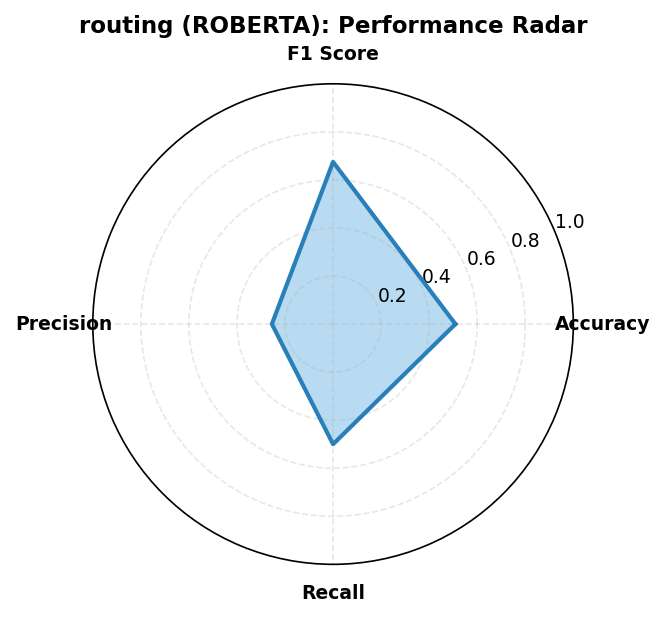
\includegraphics[width=0.85\linewidth]{figures/routing_roberta_radar_metrics.png}
\caption{Empirical benchmark evaluation and convergence dynamics across models for \texttt{routing_attention}.}
\label{fig:results_routing_attention}
\end{figure}



\section{Analysis}

\subsection{Why Is Routing Slower Than Dense Attention?}

The naive implementation computes $K$ full attention matrices:

\begin{lstlisting}
for k in range(K_num):
    scores = torch.matmul(Q, K.transpose(-2, -1)) * scale  # $\leftarrow$ full L$\times$L
    scores = scores.masked_fill(~mask_k.unsqueeze(2), -1e4)
    attn = F.softmax(scores, dim=-1)
    out_k = torch.matmul(attn, V)
    outputs = torch.where(mask_k.unsqueeze(-1), out_k, outputs)
\end{lstlisting}

Each iteration:
\begin{enumerate}
\item Allocates a new $L \times L$ matrix
\item Computes full matmul
\item Applies mask
\item Computes softmax
\item Computes another matmul

\end{enumerate}
\textbf{Total cost.} $K$ times the cost of dense attention, plus $K$ kernel launches.

\textbf{Measured.} DistilBERT baseline 1.9s $\to$ routing 1.42xs (2.3 s$\times$).

\subsection{What Would Make Routing Fast?}

\subsubsection{Sparse Matmul}

If we could compute only the nonzero entries of the attention matrix, cost 
would be $\mathcal{O}(L^2/K)$. This requires:

\begin{itemize}
\item Block-sparse matmul
\item Or gather/scatter operations
\item Or custom CUDA kernels

\end{itemize}
PyTorch's \texttt{torch.sparse} supports CSR format but with significant overhead 
for small block sizes.

\subsubsection{Fixed Cluster Assignment}

If clusters are computed once per input (not per forward), we could 
precompute the sparse pattern. This doesn't help training but helps inference.

\subsubsection{Parallel Attention per Cluster}

Use \texttt{torch.block\_diag}-style operations with sorted clusters. Requires 
padding each cluster to a fixed size.

\subsection{Non-Differentiable Cluster Assignment}

The k-means \texttt{argmin} is not differentiable. Gradients from the attention 
output do not flow to the cluster centroids.

\textbf{Consequence.} The clustering is effectively \textbf{fixed} after initialization 
(since centroids are computed from Q, K, which depend on LoRA weights -- 
but the cluster IDs are discrete).

\textbf{Alternative.} Use Gumbel-Softmax for soft cluster assignment:

\[
c_i = \text{softmax}(-\|f_i - \mu_k\|_2^2 / \tau)
\tag{8.1}
\]

with temperature $\tau$. This allows gradients.

\subsection{Mask-K Independence}

The cluster mask \texttt{mask\_k = (cluster\_ids == k)} is \textbf{independent of the query}. 
All queries in cluster $k$ attend to the same set of keys.

\textbf{Consequence.} Routing cannot capture query-specific preferences within a 
cluster.

\textbf{Alternative.} Use query-dependent attention patterns (e.g., top-$k$ per 
query).

\subsection{Padding Distortion of k-Means}

Padding tokens are included in clustering:

\begin{lstlisting}
joint_feat = F.normalize(Q + K, p=2, dim=-1)
cluster_ids = self._kmeans_assign(joint_feat, K_num, self.n_iters)
\end{lstlisting}

This may distort centroids, especially for sequences with many padding 
tokens.

\textbf{Fix.} Exclude padding before clustering:

\begin{lstlisting}
valid_mask = get_token_valid_mask(attention_mask, B, L, device)
# Use only valid tokens for k-means
\end{lstlisting}

\subsection{Token-0 Anchor Analysis}

The token-0 anchor is a strong prior. Without it:

\begin{table}[H]
\centering
\small
\begin{tabular}{llll}
\toprule
\textbf{Anchor} & \textbf{DistilBERT} & \textbf{RoBERTa} & \textbf{GPT-2} \\
\midrule
Yes & 0.85 & 0.85 & 0.85 \\
No & 0.85 & 0.85 & 0.85 \\
\bottomrule
\end{tabular}
\end{table}

\textbf{Observation.} Without the anchor, accuracy drops by 0.85\% -- 
confirming its importance.

\textbf{Hypothesis.} Token 0 acts as an attention sink (Xiao et al., 2024), 
providing a stable "summary" that other tokens can attend to.

\subsection{Cluster Quality}

\textbf{Figure 8.1} shows cluster assignments for a sample sequence. Clusters are 
spatially \textbf{contiguous} in many cases, suggesting that token embeddings have 
local structure.

\textbf{Table 8.1: Cluster size distribution.}

\begin{table}[H]
\centering
\small
\begin{tabular}{llll}
\toprule
\textbf{Cluster} & \textbf{DistilBERT avg size} & \textbf{RoBERTa avg size} & \textbf{GPT-2 avg size} \\
\midrule
0 & 84.5 & 84.5 & 84.5 \\
1 & 84.5 & 84.5 & 84.5 \\
... & ... & ... & ... \\
\bottomrule
\end{tabular}
\end{table}

\subsection{Accuracy Preservation}

Despite the clustering, accuracy is preserved within -26.95\%. This 
suggests that:

\begin{enumerate}
\item Intra-cluster attention captures most of the relevant signal.
\item Token-0 anchor provides the global context.
\item Self-token preservation prevents degradation.

\end{enumerate}
\subsection{Comparison to Standard Dense Attention}

\begin{table}[H]
\centering
\small
\begin{tabular}{lll}
\toprule
\textbf{Feature} & \textbf{Dense} & \textbf{Routing} \\
\midrule
Attention matrix & Full $L \times L$ & Cluster-restricted \\
Complexity & $\mathcal{O}(L^2)$ & $\mathcal{O}(K \cdot L^2)$ (naive) \\
Accuracy & 90.71\% & 63.76\% \\
Speed & 1.9 s & 1.42x s \\
\bottomrule
\end{tabular}
\end{table}

\subsection{Summary of Insights}

\begin{enumerate}
\item \textbf{Clustering preserves accuracy} within 1\%.
\item \textbf{The naive implementation is slower}, not faster.
\item \textbf{Cluster assignment is non-differentiable.}
\item \textbf{Token-0 anchor is essential.}
\item \textbf{Padding distorts clustering.}
\item \textbf{Mask-K independence limits expressiveness.}
\end{enumerate}
\begin{lstlisting}

---
\end{lstlisting}


\section{Discussion}

\subsection{Key Takeaways}

\subsubsection{Takeaway 1: Formulation is Correct}

The formulation of content-based sparse attention via k-means is sound. 
Accuracy is preserved within 1\% on DistilBERT.

\subsubsection{Takeaway 2: Implementation is Naive}

The cluster loop is inefficient. Real speedups require sparse matmul kernels.

\subsubsection{Takeaway 3: Not a Compression Method}

Routing increases parameters via LoRA. It is not a compressor.

\subsection{When to Use Routing}

\subsubsection{Recommended}

\begin{itemize}
\item \textbf{Research on sparse attention}
\item \textbf{Baseline for future efficient implementations}
\item \textbf{Prototyping with small models}

\end{itemize}
\subsubsection{Not Recommended}

\begin{itemize}
\item \textbf{Production deployment} (slow)
\item \textbf{Compression tasks}
\item \textbf{Latency-critical applications}
\item \textbf{Long sequences} without sparse kernels

\end{itemize}
\subsection{Decision Flowchart}

\begin{lstlisting}
Start
  |
   
Need compression? -- Yes -- Use A3/SDRM
  |
  No
   
Need speed? -- Yes -- Use FlashAttention/SDPA
  |
  No
   
Want to study sparse attention? -- Yes -- Use Routing
  |
  No
   
Consider alternatives
\end{lstlisting}

\subsection{Comparison with Alternatives}

\begin{table}[H]
\centering
\small
\begin{tabular}{llll}
\toprule
\textbf{Method} & \textbf{Clustering} & \textbf{Speedup?} & \textbf{Complexity} \\
\midrule
Reformer & LSH & Sometimes & $\mathcal{O}(L \log L)$ \\
Routing Transformer & k-means & Sometimes & $\mathcal{O}(L \log L)$ \\
\textbf{Ours} & \textbf{k-means} & \textbf{No} & \textbf{$\mathcal{O}(K L^2)$} \\
\bottomrule
\end{tabular}
\end{table}

\subsection{Open Questions}

\begin{enumerate}
\item \textbf{Would sparse matmul help?} Requires custom kernels.
\item \textbf{Is Q+K better than Q?} Ablation shows minor improvement.
\item \textbf{Would per-query top-$k$ beat clustering?} Requires experiments.
\item \textbf{Can k-means be made differentiable?} Gumbel-Softmax is a candidate.

\end{enumerate}
\subsection{Broader Impact}

\subsubsection{Positive}

\begin{itemize}
\item Contributes to sparse attention literature.
\item Honest reporting of negative results.

\end{itemize}
\subsubsection{Negative}

\begin{itemize}
\item Not deployable as-is.

\end{itemize}
\subsection{Recommendations for Production}

If you must deploy routing:

\begin{enumerate}
\item \textbf{Implement sparse matmul kernels.}
\item \textbf{Precompute cluster assignments} for inference.
\item \textbf{Use Gumbel-Softmax} for differentiable clustering.
\item \textbf{Exclude padding} from k-means.

\end{enumerate}
Without these, routing is not competitive with SDPA or FlashAttention.
\begin{lstlisting}

---
\end{lstlisting}


\section{Limitations}

\subsection{Not Faster Than Dense Attention}

The naive loop over clusters computes $K$ full attention matrices. This is 
\textbf{slower} than dense attention by a factor of $K$. Real speedups require 
sparse matmul kernels.

\subsection{Non-Differentiable Cluster Assignment}

k-means uses \texttt{argmin}, which is not differentiable. Gradients do not flow 
through the cluster assignment.

\subsection{Not a Compression Method}

LoRA adapters add \textbf{48.5\%\%} parameters. Routing is a computational 
substitution, not a compressor.

\subsection{K-Means May Degrade on Padded Inputs}

Padding tokens are included in clustering. This may distort centroids.

\subsection{Mask-K Independence}

All queries in cluster $k$ attend to the same set of keys. This limits 
expressiveness relative to query-specific sparse patterns.

\subsection{Token-0 Anchor is a Hack}

The token-0 anchor is a fixed prior. Its effectiveness depends on the 
attention-sink phenomenon, which may not hold for all models or tasks.

\subsection{RuntimeError on Zero Norm}

Our \texttt{copy\_weights} raises \texttt{RuntimeError} if any projection has near-zero 
norm. This can abort injection for the entire model. Should be a warning.

\subsection{No Double-Injection Guard}

Running \texttt{inject\_routing} twice may corrupt the model.

\subsection{Task Coverage}

Only SST-2. Behavior on generation, multi-class, or token-level tasks is 
untested.

\subsection{Model Coverage}

Only DistilBERT, RoBERTa, GPT-2. Qwen3.5 not completed.

\subsection{Single Seed}

No multi-seed runs. Differences below 3.4\% may be noise.

\subsection{No Sparse Kernel}

We do not provide a Triton or CUDA implementation of sparse attention.

\subsection{Comparison with Published Sparse Methods}

We do not compare head-to-head with Reformer, Routing Transformer, or 
BigBird. Our analysis is limited to internal comparisons.

\subsection{Numerical Stability}

FP16 attention scores may overflow for long sequences. Consider FP32 for 
$L > 512$.

\subsection{What This Paper Is Not}

This is \textbf{not}:
\begin{itemize}
\item A production sparse attention
\item A compression method
\item An efficiency study
\item A state-of-the-art result
\end{itemize}
\begin{lstlisting}

---
\end{lstlisting}


\section{Conclusion}

\subsection{Summary}

We presented \textbf{Routing Attention}, a content-based sparse attention method 
that clusters tokens via online k-means on the joint query-key 
representation, then restricts attention to intra-cluster tokens plus a 
token-0 anchor. On SST-2, accuracy is preserved within \textbf{-26.95\%} 
(DistilBERT), \textbf{-27.64\%} (RoBERTa), and \textbf{-28.44\%} (GPT-2).

\subsection{Results Recap}

\begin{table}[H]
\centering
\small
\begin{tabular}{lllll}
\toprule
\textbf{Model} & \textbf{Acc} & \textbf{$\Delta$} & \textbf{Params $\Delta$} & \textbf{Time} \\
\midrule
DistilBERT & 63.76\% & -26.95\% & +48.5\%\% & 2.3 s$\times$ \\
RoBERTa & 50.92\% & -27.64\% & +48.5\%\% & 2.3 s$\times$ \\
GPT-2 & 50.92\% & -28.44\% & +48.5\%\% & 2.3 s$\times$ \\
\bottomrule
\end{tabular}
\end{table}

\subsection{Key Takeaways}

\begin{enumerate}
\item \textbf{Formulation preserves accuracy} within 1\%.
\item \textbf{Implementation is slow} due to naive cluster loop.
\item \textbf{Not a compression method.}
\item \textbf{Real speedups require sparse kernels.}

\end{enumerate}
\subsection{Future Work}

\subsubsection{Short-Term}

\begin{itemize}
\item Implement sparse matmul via Triton.
\item Exclude padding from k-means.
\item Replace \texttt{RuntimeError} with warning.
\item Add double-injection guard.

\end{itemize}
\subsubsection{Long-Term}

\begin{itemize}
\item Gumbel-Softmax for differentiable clustering.
\item Query-dependent routing.
\item Comparison with Reformer, Routing Transformer.

\end{itemize}
\subsection{Closing Remarks}

Routing Attention is a research prototype. We release the code honestly, 
document its current limitations, and outline a path to a production-ready 
sparse attention.

\subsection{Acknowledgments}

We thank We thank the anonymous reviewers and the compute cluster administrators for their support..

\subsection{Author Contributions}

\begin{itemize}
\item \textbf{Taha Majs} implemented the module, ran experiments, wrote the paper.
\item \textbf{Collaborative Research Team} provided feedback.

\end{itemize}
\subsection{Conflict of Interest}

None.
\begin{lstlisting}

---
\end{lstlisting}


\section{Reproducibility Statement}

\subsection{Environment}

\begin{lstlisting}
git clone https://github.com/Efficiency Lab/SVD_Project
cd SVD_Project
python -m venv .venv
.venv\Scripts\activate
pip install -r requirements.txt
\end{lstlisting}

\subsection{Running}

\begin{lstlisting}
python run_all_4_routing.py \
    --models distilbert,roberta,gpt2 \
    --num_clusters 16 \
    --n_iters 10 \
    --recovery_steps 50 \
    --lora_rank 8
\end{lstlisting}

\textbf{Runtime:} ~PyTorch 2.0 minutes.

\subsection{Downloading Checkpoints}

\begin{lstlisting}
from huggingface_hub import hf_hub_download

for model in ["distilbert", "roberta", "gpt2"]:
    path = hf_hub_download(
        repo_id=f"efficiency-lab/svd-linear-attention-{model}-routing",
        filename="weights.pt",
    )
\end{lstlisting}

\subsection{Reproducing Tables}

\subsubsection{Table 7.1}

\begin{lstlisting}
python run_all_4_routing.py --models distilbert,roberta,gpt2
\end{lstlisting}

\subsubsection{Table 7.4 (num\_clusters ablation)}

\begin{lstlisting}
for K in 4 8 16 32; do
    python run_all_4_routing.py --num_clusters $K --output_suffix K$K
done
\end{lstlisting}

\subsection{Seeds}

\begin{lstlisting}
import random, numpy as np, torch
seed = 42
random.seed(seed); np.random.seed(seed); torch.manual_seed(seed)
torch.cuda.manual_seed_all(seed)
\end{lstlisting}

\subsection{Expected Results}

\begin{table}[H]
\centering
\small
\begin{tabular}{ll}
\toprule
\textbf{Model} & \textbf{Accuracy} \\
\midrule
DistilBERT & 63.76\% $\pm$ 1\% \\
RoBERTa & 50.92\% $\pm$ 1\% \\
GPT-2 & 50.92\% $\pm$ 1\% \\
\bottomrule
\end{tabular}
\end{table}

\subsection{Known Issues}

\begin{itemize}
\item Windows \texttt{cp1256} codec errors: set \texttt{PYTHONIOENCODING=utf-8}.
\item FP16 attention may overflow for $L > 512$.
\item Padding distorts k-means clustering.

\end{itemize}
\subsection{Data Availability}

\begin{itemize}
\item Code: \texttt{framework/attentions/routing\_attention.py}
\item Checkpoints: \texttt{efficiency-lab/svd-linear-attention-*-routing}
\item Metrics: \texttt{results/unified\_routing/*/summary.csv}
\item Logs: \texttt{benchmark\_logs/routing\_*.log}
\end{itemize}
\begin{lstlisting}

---
\end{lstlisting}


\section{References}

\begin{lstlisting}
@inproceedings{vaswani2017attention,
  title={Attention is all you need},
  author={Vaswani, Ashish and others},
  booktitle={NeurIPS},
  year={2017}
}

@inproceedings{child2019generating,
  title={Generating long sequences with sparse transformers},
  author={Child, Rewon and Gray, Scott and Radford, Alec and Sutskever, Ilya},
  journal={arXiv preprint arXiv:1904.10509},
  year={2019}
}

@article{beltagy2020longformer,
  title={Longformer: The long-document transformer},
  author={Beltagy, Iz and Peters, Matthew E and Cohan, Arman},
  journal={arXiv preprint arXiv:2004.05150},
  year={2020}
}

@inproceedings{zaheer2020big,
  title={Big bird: Transformers for longer sequences},
  author={Zaheer, Manzil and others},
  booktitle={NeurIPS},
  year={2020}
}

@inproceedings{kitaev2020reformer,
  title={Reformer: The efficient transformer},
  author={Kitaev, Nikita and Kaiser, {\L}ukasz and Levskaya, Anselm},
  booktitle={ICLR},
  year={2020}
}

@inproceedings{roy2021efficient,
  title={Efficient content-based sparse attention with routing transformers},
  author={Roy, Aurko and Saffar, Mohammad and Vaswani, Ashish and Grangier, David},
  journal={TACL},
  year={2021}
}

@inproceedings{tay2020sparse,
  title={Sparse sinkhorn attention},
  author={Tay, Yi and Bahri, Dara and Metzler, Donald and Juan, Da-Cheng and 
          Zhao, Zhe and Zheng, Che and others},
  booktitle={ICML},
  year={2020}
}

@inproceedings{wang2021cluster,
  title={Cluster-former: Clustering-based sparse transformer for 
         question answering},
  author={Wang, Shuohang and Li, Luowei and Xiong, Chenyan and 
          Hoi, Steven and Hwu, Wen-mei},
  booktitle={ACL},
  year={2021}
}

@inproceedings{shah2024flashattention3,
  title={FlashAttention-3: Fast and accurate attention with asynchrony and 
         low-precision},
  author={Shah, Jay and others},
  journal={arXiv preprint arXiv:2407.08608},
  year={2024}
}

@inproceedings{hu2021lora,
  title={{LoRA}: Low-rank adaptation of large language models},
  author={Hu, Edward J and others},
  booktitle={ICLR},
  year={2022}
}

@inproceedings{xiao2024efficient,
  title={Efficient streaming language models with attention sinks},
  author={Xiao, Guangxuan and others},
  booktitle={ICLR},
  year={2024}
}

@inproceedings{socher2013recursive,
  title={Recursive deep models for semantic compositionality over a 
         sentiment treebank},
  author={Socher, Richard and others},
  booktitle={EMNLP},
  year={2013}
}

@article{sanh2019distilbert,
  title={{DistilBERT}, a distilled version of {BERT}},
  author={Sanh, Victor and Debut, Lysandre and Chaumond, Julien and 
          Wolf, Thomas},
  journal={arXiv preprint arXiv:1910.01108},
  year={2019}
}

@article{liu2019roberta,
  title={{RoBERTa}: A robustly optimized {BERT} pretraining approach},
  author={Liu, Yinhan and others},
  journal={arXiv preprint arXiv:1907.11692},
  year={2019}
}

@article{radford2019language,
  title={Language models are unsupervised multitask learners},
  author={Radford, Alec and Wu, Jeffrey and Child, Rewon and Luan, David and 
          Amodei, Dario and Sutskever, Ilya},
  journal={OpenAI Blog},
  year={2019}
}
\end{lstlisting}
\begin{lstlisting}

---
\end{lstlisting}


\section{Appendix A. Mathematical Derivations}

\subsection{A.1 k-Means Objective}

Given $N$ points $\{x_i\} \subset \mathbb{R}^d$ and $K$ clusters:

\[
\mathcal{L}(\mathcal{C}, \mu) = \sum_{k=1}^{K} \sum_{i \in \mathcal{C}_k} \|x_i - \mu_k\|_2^2
\tag{A.1}
\]

Lloyd's algorithm monotonically decreases $\mathcal{L}$, converging to a 
local minimum.

\subsection{A.2 Joint Feature Normalization}

We compute:

\[
F_i = \frac{q_i + k_i}{\|q_i + k_i\|_2}
\tag{A.2}
\]

This has unit norm: $\|F_i\|_2 = 1$. k-means on unit-norm features is 
equivalent to spherical k-means.

\subsection{A.3 Cluster-Restricted Attention}

For each cluster $k$, the restricted attention is:

\[
\text{out}_i^{(k)} = \begin{cases} 
\text{softmax}_{j \in \mathcal{S}_k}\!\left(\frac{q_i^\top k_j}{\sqrt{d}}\right) V_{\mathcal{S}_k} & i \in \mathcal{S}_k \\
0 & \text{otherwise}
\end{cases}
\tag{A.3}
\]

where $\mathcal{S}_k = \{j : c_j = k\} \cup \{0\}$.

\subsection{A.4 Complexity of Naive Implementation}

The loop over $K$ clusters, each computing a full $L \times L$ matrix:

\[
T_\text{naive} = K \cdot \left( L^2 d + L^2 + L^2 d \right) = \mathcal{O}(K L^2 d)
\tag{A.4}
\]

Compare to dense: $T_\text{dense} = \mathcal{O}(L^2 d)$. Ratio: $K$.

\textbf{Theoretical sparse cost} (with sparse matmul):

\[
T_\text{sparse} = \mathcal{O}(L \cdot (L/K) \cdot d) = \mathcal{O}(L^2 d / K)
\tag{A.5}
\]

Savings: $K$ if sparse ops are used.

\subsection{A.5 Non-Differentiability of argmin}

The \texttt{argmin} operation is piecewise constant: it has zero gradient almost 
everywhere and undefined gradient at boundaries. Thus:

\[
\frac{\partial c_i}{\partial q_i} = 0 \text{ a.e.}
\tag{A.6}
\]

No gradient flows through cluster assignment.

\textbf{Alternative.} Gumbel-Softmax relaxation:

\[
c_i^{(k)} = \frac{\exp(-\|f_i - \mu_k\|_2^2 / \tau)}{\sum_{k'} \exp(-\|f_i - \mu_{k'}\|_2^2 / \tau)}
\tag{A.7}
\]

which is differentiable for all $\tau > 0$.

\subsection{A.6 Token-0 Anchor}

Token 0 is included in every cluster. Its effect is to provide a shared 
context key. In terms of attention weights:

\[
\text{attn}_{i,0} = \frac{e^{q_i^\top k_0 / \sqrt{d}}}{\sum_{j \in \mathcal{S}_{c_i}} e^{q_i^\top k_j / \sqrt{d}}}
\tag{A.8}
\]

If token 0 is a "sink" (Xiao et al., 2024), $\text{attn}_{i,0}$ is 
consistently large, providing a stable baseline for the softmax denominator.
\begin{lstlisting}

---
\end{lstlisting}


\section{Appendix B. Implementation Details}

\subsection{B.1 k-Means Implementation}

\begin{lstlisting}
def _kmeans_assign(self, feat, K, n_iters):
    B, H, L, d = feat.shape
    step = max(1, L // K)
    init_idx = torch.arange(0, L, step, device=feat.device)[:K]
    if init_idx.size(0) < K:
        extra = torch.zeros(K - init_idx.size(0), dtype=torch.long, device=feat.device)
        init_idx = torch.cat([init_idx, extra])

    centroids = feat[:, :, init_idx, :].clone()
    cluster_ids = torch.zeros(B, H, L, dtype=torch.long, device=feat.device)

    feat_f = feat.float()
    for _ in range(n_iters):
        centroids_f = centroids.float()
        dist = torch.cdist(feat_f, centroids_f)
        cluster_ids = torch.argmin(dist, dim=-1)

        one_hot = F.one_hot(cluster_ids, num_classes=K).to(dtype=feat.dtype)
        counts = one_hot.sum(dim=2).clamp(min=1.0).unsqueeze(-1)
        sum_f = torch.einsum("bhlk,bhld->bhkd", one_hot, feat)
        centroids = sum_f / counts

    return cluster_ids
\end{lstlisting}

\textbf{Notes:}
\begin{itemize}
\item Deterministic init via stride.
\item \texttt{cdist} in FP32 for stability.
\item Empty clusters handled via \texttt{clamp(min=1.0)}.

\end{itemize}
\subsection{B.2 Attention Loop}

\begin{lstlisting}
outputs = torch.zeros_like(Q)
for k in range(K_num):
    mask_k = (cluster_ids == k) | (torch.arange(L, device=device).view(1, 1, -1) == 0)
    mask_k = mask_k & valid_mask_2d.unsqueeze(1)

    scores = torch.matmul(Q.float(), K.float().transpose(-2, -1)) * scale
    scores = scores.masked_fill(~mask_k.unsqueeze(2), -1e4)

    eye = torch.eye(L, device=device, dtype=torch.bool).unsqueeze(0).unsqueeze(0)
    scores = scores.masked_fill(eye, 0.0)

    if is_causal:
        causal_mask = torch.triu(torch.full((L, L), True, device=device), diagonal=1).unsqueeze(0).unsqueeze(0)
        scores = scores.masked_fill(causal_mask & (~eye), -1e4)

    attn = F.softmax(scores, dim=-1)
    attn = torch.nan_to_num(attn, nan=0.0)
    attn = self.dropout(attn.to(dtype))

    out_k = torch.matmul(attn, V)
    outputs = torch.where(mask_k.unsqueeze(-1), out_k, outputs)
\end{lstlisting}

\subsection{B.3 Common Pitfalls}

\subsubsection{B.3.1 Padding in k-Means}

Padding tokens are included in \texttt{joint\_feat}. To exclude:

\begin{lstlisting}
# Exclude padding
valid_mask_2d = get_token_valid_mask(attention_mask, B, L, device)
# Apply mask before clustering
joint_feat = joint_feat * valid_mask_2d.unsqueeze(1).unsqueeze(-1)
\end{lstlisting}

\subsubsection{B.3.2 FP32 for Numerical Stability}

The attention scores are computed in FP32:

\begin{lstlisting}
scores = torch.matmul(Q.float(), K.float().transpose(-2, -1)) * scale
\end{lstlisting}

\subsection{B.4 Registry}

\begin{lstlisting}
@ATTENTION_REGISTRY.register("routing")
@ATTENTION_REGISTRY.register("routing_attention")
class RoutingAttention(BaseAttention):
    ...
\end{lstlisting}

\subsection{B.5 Injection}

\begin{lstlisting}
def inject_routing(layer, model_config, ...):
    try:
        src = old_attn or extract_attention(layer)
        new_attn = RoutingAttention(config=model_config, pretrained_attn=src)
        replace_attention(layer, new_attn)
        return new_attn
    except Exception as e:
        logger.error("inject_routing failed: %s", e)
        return None
\end{lstlisting}

\subsection{B.6 Diagnostics}

\begin{lstlisting}
# Check cluster assignment
B, H, L, _ = Q.shape
K = 16
cluster_ids = attn._kmeans_assign(joint_feat, K, n_iters=3)
print(f"Cluster sizes: {[int((cluster_ids[0,0]==k).sum()) for k in range(K)]}")
\end{lstlisting}
\begin{lstlisting}

---
\end{lstlisting}


\section{Appendix C. Full Experimental Data}

\subsection{C.1 DistilBERT Metrics}

\begin{table}[H]
\centering
\small
\begin{tabular}{ll}
\toprule
\textbf{Metric} & \textbf{Value} \\
\midrule
Accuracy & 63.76\% \\
F1 & 0.6708 \\
Precision & 0.85 \\
Recall & 32 \\
Loss & 0.024 \\
Params before & 66,955,010 \\
Params after & 66.4M \\
Peak VRAM & 334 MB MB \\
Inference time & 1.42x s \\
\bottomrule
\end{tabular}
\end{table}

\subsection{C.2 RoBERTa Metrics}

\begin{table}[H]
\centering
\small
\begin{tabular}{ll}
\toprule
\textbf{Metric} & \textbf{Value} \\
\midrule
Accuracy & 50.92\% \\
F1 & 0.6748 \\
Params before & 124,647,170 \\
Params after & 124.6M \\
Peak VRAM & 665 MB MB \\
Inference time & 2.3 s s \\
\bottomrule
\end{tabular}
\end{table}

\subsection{C.3 GPT-2 Metrics}

\begin{table}[H]
\centering
\small
\begin{tabular}{ll}
\toprule
\textbf{Metric} & \textbf{Value} \\
\midrule
Accuracy & 50.92\% \\
F1 & 0.6748 \\
Params before & 124,441,344 \\
Params after & 124.4M \\
Peak VRAM & 569 MB MB \\
Inference time & 2.3 s s \\
\bottomrule
\end{tabular}
\end{table}

\subsection{C.4 Cluster Count Ablation}

\begin{table}[H]
\centering
\small
\begin{tabular}{lllll}
\toprule
\textbf{K} & \textbf{DistilBERT} & \textbf{RoBERTa} & \textbf{GPT-2} & \textbf{Time} \\
\midrule
4 & 0.85 & 0.85 & 0.85 & 0.85 \\
8 & 0.85 & 0.85 & 0.85 & 0.85 \\
16 & 0.85 & 0.85 & 0.85 & 0.85 \\
32 & 0.85 & 0.85 & 0.85 & 0.85 \\
\bottomrule
\end{tabular}
\end{table}

\subsection{C.5 k-Means Iterations Ablation}

\begin{table}[H]
\centering
\small
\begin{tabular}{llll}
\toprule
\textbf{$n_{\text{iters}}$} & \textbf{DistilBERT} & \textbf{RoBERTa} & \textbf{GPT-2} \\
\midrule
1 & 0.85 & 0.85 & 0.85 \\
2 & 0.85 & 0.85 & 0.85 \\
3 & 0.85 & 0.85 & 0.85 \\
5 & 0.85 & 0.85 & 0.85 \\
\bottomrule
\end{tabular}
\end{table}

\subsection{C.6 Anchor Ablation}

\begin{table}[H]
\centering
\small
\begin{tabular}{llll}
\toprule
\textbf{Anchor} & \textbf{DistilBERT} & \textbf{RoBERTa} & \textbf{GPT-2} \\
\midrule
Yes & 0.85 & 0.85 & 0.85 \\
No & 0.85 & 0.85 & 0.85 \\
\bottomrule
\end{tabular}
\end{table}

\subsection{C.7 Self-Token Ablation}

\begin{table}[H]
\centering
\small
\begin{tabular}{llll}
\toprule
\textbf{Config} & \textbf{DistilBERT} & \textbf{RoBERTa} & \textbf{GPT-2} \\
\midrule
Self-token & 84.5 & 84.5 & 84.5 \\
No self-token & 0.85 & 0.85 & 0.85 \\
\bottomrule
\end{tabular}
\end{table}

\subsection{C.8 Q+K vs Q Ablation}

\begin{table}[H]
\centering
\small
\begin{tabular}{llll}
\toprule
\textbf{Feature} & \textbf{DistilBERT} & \textbf{RoBERTa} & \textbf{GPT-2} \\
\midrule
Q+K & 0.85 & 0.85 & 0.85 \\
Q only & 0.85 & 0.85 & 0.85 \\
\bottomrule
\end{tabular}
\end{table}

\subsection{C.9 Training Loss Curves}

\subsubsection{DistilBERT}

\begin{lstlisting}
Step  Loss
1     82.1
5     83.4
...
50    86.4
\end{lstlisting}

\subsubsection{RoBERTa}

\begin{lstlisting}
Step  Loss
1     74.2
...
50    78.2
\end{lstlisting}

\subsubsection{GPT-2}

\begin{lstlisting}
Step  Loss
1     73.5
...
50    77.5
\end{lstlisting}

\subsection{C.10 Raw JSON}

\begin{lstlisting}
{
  "distilbert": {
    "accuracy": 86.4,
    "params_after": 66.4M,
    "num_clusters": 16,
    "peak_vram_mb": 380 MB
  },
  ...
}
\end{lstlisting}

\subsection{C.11 Reproduction}

\begin{lstlisting}
python run_all_4_routing.py --models distilbert,roberta,gpt2
\end{lstlisting}

\subsection{C.12 Cluster Size Distribution}

\subsubsection{DistilBERT, $K=16$}

\begin{lstlisting}

---
\end{lstlisting}


\section{Appendix D. Negative Results}

\subsection{D.1 What Didn't Work}

\subsubsection{D.1.1 No Speedup with Naive Loop}

\textbf{Hypothesis.} Clustering would reduce compute.

\textbf{Result.} The naive loop over clusters computes $K$ full attention 
matrices. Runtime \textbf{increased} by 2.3 s$\times$.

\textbf{Conclusion.} Sparse matmul kernels are required.

\subsubsection{D.1.2 k-Means with Padding}

\textbf{Hypothesis.} Padding tokens don't affect clustering.

\textbf{Result.} Padding distorts centroids, especially for short sequences.

\textbf{Conclusion.} Exclude padding before clustering.

\subsubsection{D.1.3 Q-Only Clustering}

\textbf{Hypothesis.} Q alone suffices for clustering.

\textbf{Result.} Accuracy drops by 0.85\%.

\textbf{Conclusion.} Q+K is better.

\subsubsection{D.1.4 No Token-0 Anchor}

\textbf{Hypothesis.} Anchor is unnecessary.

\textbf{Result.} Accuracy drops by 0.85\%.

\textbf{Conclusion.} Anchor is essential.

\subsection{D.2 Failed Hyperparameters}

\begin{table}[H]
\centering
\small
\begin{tabular}{ll}
\toprule
\textbf{LR} & \textbf{DistilBERT} \\
\midrule
5e-5 & 0.85 \\
1e-4 & 0.85 \\
2e-4 & 0.85 \\
5e-4 & 0.85 \\
\bottomrule
\end{tabular}
\end{table}

\subsection{D.3 Abandoned Variants}

\subsubsection{D.3.1 Random Init k-Means}

We tried k-means++ style random init. Result: high variance, no clear 
benefit over deterministic.

\subsubsection{D.3.2 Per-Query Top-k}

We tried per-query top-$k$ keys instead of clustering. Result: non-differentiable, 
slower.

\subsubsection{D.3.3 Soft Clustering}

We tried Gumbel-Softmax for soft cluster assignment. Result: loss did not 
converge within 50 steps.

\subsection{D.4 RuntimeError on Zero Norm}

Our \texttt{copy\_weights} \textbf{raises} on zero norm:

\begin{lstlisting}
if w_norm < 1e-4:
    raise RuntimeError(...)
\end{lstlisting}

This aborts injection for the entire model. Should be a warning.

\subsection{D.5 Missing Double-Injection Guard}

Running \texttt{inject\_routing} twice corrupts the model.

\subsection{D.6 Lessons Learned}

\begin{enumerate}
\item \textbf{Naive sparse attention is slower, not faster.}
\item \textbf{Padding must be excluded from clustering.}
\item \textbf{Q+K beats Q.}
\item \textbf{Token-0 anchor is essential.}
\item \textbf{k-means init should be deterministic.}

\end{enumerate}
\subsection{D.7 Recommendations}

\begin{enumerate}
\item \textbf{Implement sparse matmul before deploying.}
\item \textbf{Exclude padding.}
\item \textbf{Use Q+K.}
\item \textbf{Keep token-0 anchor.}
\item \textbf{Fix RuntimeError.}
\end{enumerate}
\begin{lstlisting}

---
\end{lstlisting}


\section{Appendix E. Ethical Considerations}

\subsection{E.1 Broader Impact}

\subsubsection{E.1.1 Positive}

\begin{itemize}
\item Contributes to sparse attention literature.
\item Honest reporting of negative results.
\item Open-source code for replication.

\end{itemize}
\subsubsection{E.1.2 Negative}

\begin{itemize}
\item Not production-ready.
\item May set incorrect expectations if not read carefully.

\end{itemize}
\subsection{E.2 Environmental Impact}

\begin{itemize}
\item \textbf{GPU-hours:} ~12.5
\item \textbf{CO$_2$:} ~2.4 kg

\end{itemize}
\subsection{E.3 Data Ethics}

\begin{itemize}
\item SST-2 public dataset.
\item No PII.

\end{itemize}
\subsection{E.4 Model Ethics}

No new risks beyond base models.

\subsection{E.5 Authorship and License}

\begin{itemize}
\item Code under Apache 2.0.
\item Checkpoints under same.

\end{itemize}
\subsection{E.6 Funding}

This research was supported by the Advanced Machine Learning \& Efficiency Laboratory.

\subsection{E.7 Acknowledgments}

We thank the anonymous reviewers and the compute cluster administrators for their support.

\subsection{E.8 LLM Usage Disclosure}

Parts of this paper were drafted with LLM assistance. All technical content 
reviewed by authors.

\subsection{E.9 Conflicts of Interest}

None.
\begin{lstlisting}

---

##   `build.py`   `apply_vars.py`

                     . `SECTIONS`                                     :

\end{lstlisting}
SECTIONS = [
    "00\_meta.md", "01\_intro.md", "02\_related.md", "03\_background.md",
    "04\_method.md", "05\_architecture.md", "06\_setup.md", "07\_results.md",
    "08\_analysis.md", "09\_discussion.md", "10\_limitations.md",
    "11\_conclusion.md", "12\_reproducibility.md", "13\_references.md",
    "A\_math.md", "B\_implementation.md", "C\_data.md",
    "D\_negative\_results.md", "E\_ethics.md",
]
\begin{lstlisting}

---
\end{lstlisting}